Let's consider the experimental implementation of the \eqref{9:model} system in \cite{Choi_2016} with approximately unity filled Mott insulator of bosonic ${}^{87}$Rb atoms in a single plane of a cubic optical lattic. 


To do this, by combining laser beams, we will obtain a certain interference pattern, the antinodes of which, at red detuning, will act as minima of the potential for atoms due to their polarizability (an alternative would be a lattice of optical tweeters). Between these potential minima, atoms will tunnel with a characteristic energy $J$ (as in fig. \ref{fig:1Dmain}c), which we will use as an energy scale. We can adjust the interaction $U$ between atoms using Feischbach resonances, by turning it up to the value $U=24J$ we get a system close to hard-bosons. We will apply a global harmonic potential on top of the grating, also by focusing the laser. Let's fill the trap with sufficiently cold atoms, using a microwave knife, leave only the left half filled and wait a little (fig. \ref{fig:loc2D1}). Noises $\Delta$ are added to the system using DMD (alternatively, SLM, AOD or quasi-random potential are used as in \cite{schreiber_observation_2015}, more details in \cite{abanin_many-body_2019}), the result is averaged over 50 implementations of $\delta_j$.

\begin{figure}[h]
    \centering
    \addletter{80}{a}
    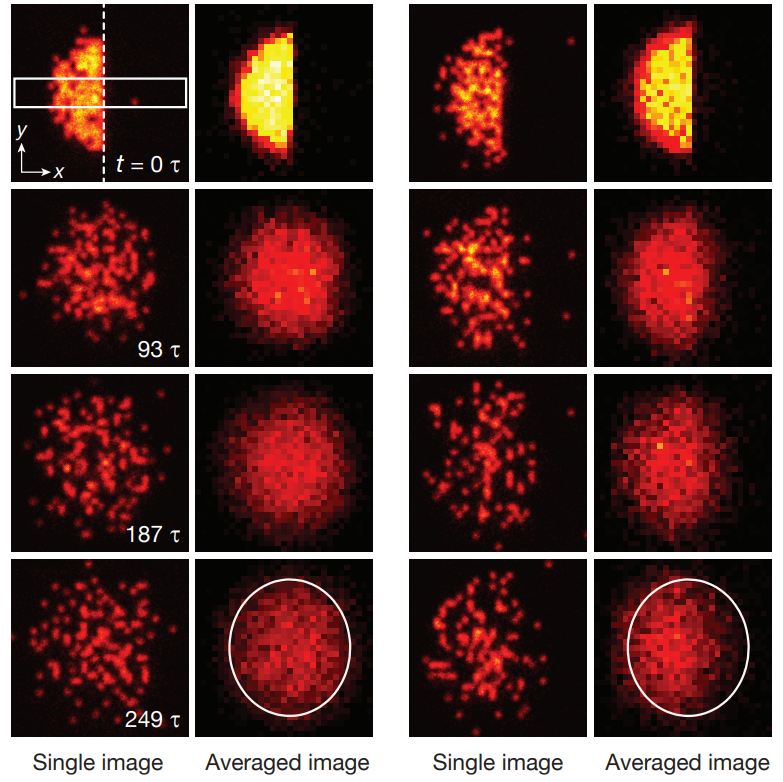
\includegraphics[align=c, width=0.33\textwidth]{imgs/MBL_2D_exp_1.png}
    \hspace{10 mm} 
    \addletter{80}{b}
    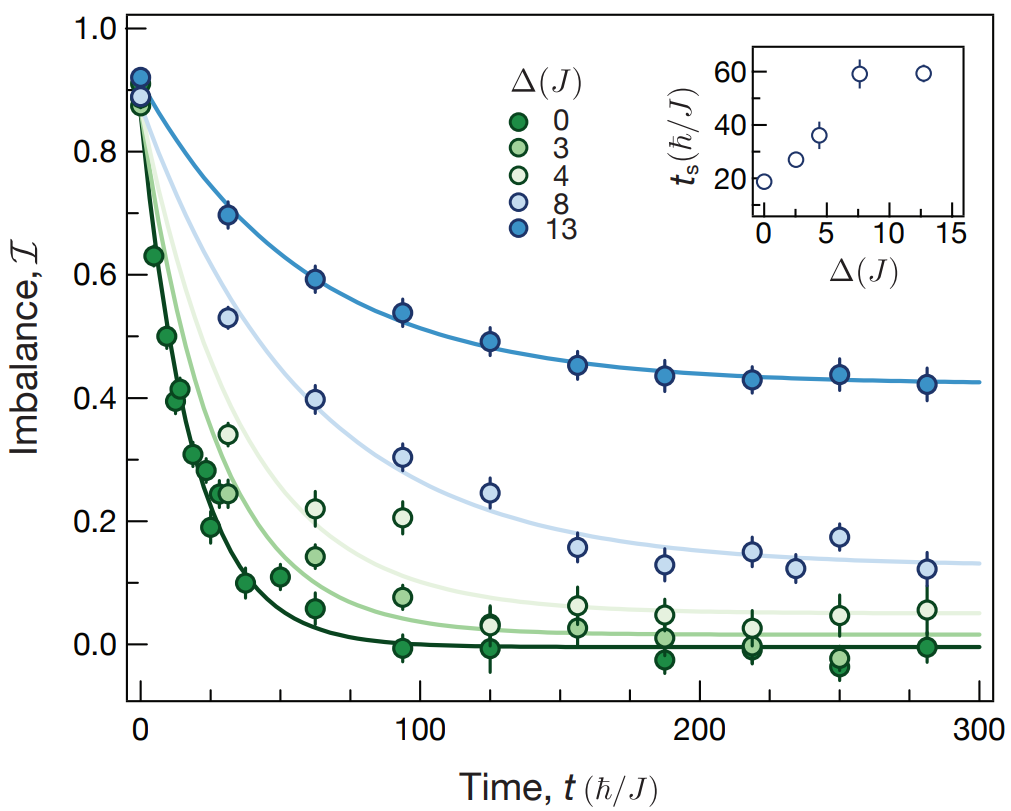
\includegraphics[align=c, width=0.4\textwidth]{imgs/MBL_2D_exp_2.png}
    % 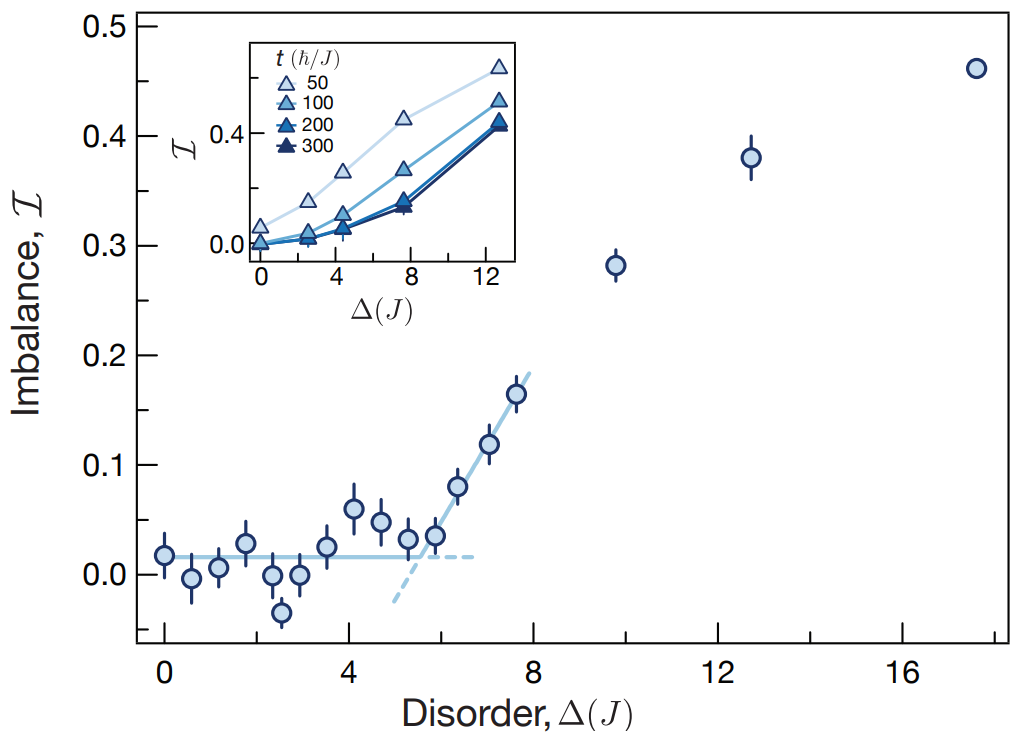
\includegraphics[align=c, width=0.4\textwidth]{imgs/MBL_2D_exp_3.png}
    \caption{
        \cite{Choi_2016}
        a) Raw fluorescence images (red to yellow corresponds to increasing detected light level) showing the evolution of the initial density step without disorder. The left column shows the evolution with $\Delta=0$ and the right column $\Delta = 13 J$.
        b) Relaxation dynamics of a density domain wall.
    }
    \label{fig:loc2D1}
\end{figure}


It can be seen that in the absence of noise the system reaches a thermal state - thermalization ($\mathcal{I} \to 0$). With sufficiently strong noise, localization occurs: $\mathcal{I}(t \to \infty) = \mathcal{I}_\infty > 0$. Assuming the output to $\mathcal{I}_\infty$ to be exponential, we can notice how what is required to reach a steady state increases as the noise level increases.


It can also be seen that $\mathcal{I}_\infty > 0$ appears with $\sub{\Delta}{c} \approx 5.5(4) J$. The article emphasizes that $\sub{\Delta}{c}$ will increase as initial filling decreases. The clear difference in critical disorder strengths highlights the strong influence of interactions on the localization.


